\subsection{Ampersand knowledge}\label{subsection:ampersand-knowledge}

When we start working with Ampersand, a development environment must first be set up.
The preferred configuration is done using Docker.
If you have little or no knowledge of Docker, you can choose to set up \acrshort{x}.
Ampersand its documentation assumes that \acrshort{x}~\footnote{\url{https://github.com/AmpersandTarski/documentation/blob/master/installing-ampersand/installing-the-tools-manually.md}} can be used for this configured.
Failed to get the local \acrshort{x} installation working using the documentation.
However, with help, we managed to get it working in the Docker environment.
So starting with Ampersand, it is not just Ampersand that needs to be studied, but also the environment where it operates in that needs to be studied.
Further setting up the environment and Ampersand also works fine from the Ampersand website and from Github.
There is also some information about Ampersand on Stackoverflow~\footnote{\url{https://stackoverflow.com/search?q=Ampersandtarski}}, but nothing else can be found outside of some scientific articles, such as~\cite{de_swart_ampersand_2011} explaining Ampersand.

The sub-question "\acrlong{RQ1}" examines the knowledge of the software engineer when using Ampersand.
To answer this question we use the links as showed in table~\ref{tab:results_to_rq}.
The categories are again clustered according to the following aggregated topics. In this respect \nameref{subsub:1_annotation}, \nameref{subsub:1_authorization_mechanism}, \nameref{subsub:1_conventions}, \nameref{subsub:1_diligence}, \nameref{subsub:1_documentation}, \nameref{subsub:1_includes}, \nameref{subsub:1_knowledge}, \nameref{subsub:1_other_knowledge}, \nameref{subsub:1_refactoring} and \nameref{subsub:1_shared_components}.

\subsubsection{Knowledge}\label{subsub:1_knowledge}
In order to be able to use Ampersand, in addition to knowledge about the structure of the environment, knowledge of Ampersand itself is required.
There is not a lot of information about Ampersand on the internet and there are examples, but they do not cover the whole load.
As with any tool and method, knowledge will have to be kept up to date to keep Ampersand usable.
This is not specific to Ampersand, but of course also applies to Ampersand.
(Ref. to \nameref{s:1_1_setup})


\subsubsection{Documentation}\label{subsub:1_documentation}
Proper use of Ampersand requires proper documentation setup.
This setup consists of knowledge of the way Ampersand handles the information in the scripts.
The positioning of the meaning of the Terms and the Relationships and the purpose of the Rule and the use of includes.
One should be aware that the meaning, purpose and definitions appear directly in the documentation and the inclusions help determine the order of the story and that this should be a unifying story.
Agreement must be reached in advance about the structure of the spelling, the reference to legislation and regulations.
The notation method, the naming convention of Concepts and Relations must also be unambiguous in order to have a consistent and professional appearance.
As one of the interviewees pointed out, when analysis and documentation needs to be done, why not through Ampersand.
Unfortunately, the researcher started to standardize somewhat later, so that this was not implemented everywhere.
(Ref. to \nameref{s:1_1_setup}, \nameref{s:1_2_script_creation})


\subsubsection{Annotation}\label{subsub:1_annotation}
When you work with the Ampersand method, the text is looped. It seems logical to process the text chronologically.
However, this will not always work, because you will have to jump back and forth in the text and a method must therefore be found to maintain the overview.
Keeping an overview is difficult when using Ampersand because the resource can be huge.
This aspect has been tested in several ways.
The XML source text has been looked at with the intention of adding additional XML tags.
The intended side effect of this was that we could generate the model from the XML.
This did not work because the original XML is too complex and would also make the XML parsing very complex and the work has to be done again with a new version of the law.
The law text could also be downloaded as RTF format. The RTF format was like a Word document and could be commented on.
The same was true for the PDF format.
\F{Annotation}{An annotation tool is needed to keep an overview of the text to be processed.
This prevents things from being processed twice or not.} within the PDF is also possible and you can also underline with colors.
Ultimately, the old-fashioned choice was made for the combination of hardcopy and the PDF.
Hardcopy for stripes and writing and the PDF for searching and copying text.
(See \nameref{s:1_3_source_handling})


\subsubsection{Refactoring}\label{subsub:1_refactoring}
Maintaining the overview in the created scripts is also a challenge.
By using Visual Studio\footnote{\acrlong{vsc} no direct involvement with Ampersand}  there are no \F{refactor}{There is a need to enable refactoring within an IDE.
We can then prevent issues when removing, for example, Includes.
Changing naming or viewing where a Concept or Relation occurs is highly desirable.} options.
Visual Studio also seems to lack integration between the scripts.
The consequence of this is that it is possible that the same Concepts and also Relationships are defined in several places.
By not being aware of the overlap, a different definition can occur for the same Concept.
The differences will not be very large, but certainly worded differently.
This only came to light when the documentation was generated.
The advantage of working with text and generating the model from it appears to be a disadvantage here.
(Ref. to \nameref{s:2_4_concept_reuse}, \nameref{s:3_2_common_objects})

\subsubsection{Diligence}\label{subsub:1_diligence}
When creating a script where the analyst does not yet have that much experience, it happens that the meaning and purpose are not filled in.
This is caused by the analyst being too busy getting Relations and Rules working within the scripts.
The consequence of this is that meanings and purposes are not filled in and they therefore become visible in the \acrshort{ca}.
It is almost impossible to update it afterwards.
This can be prevented by working as a team, where the team members keep each other sharp on these matters and there is experience in the team.
(Ref. to \nameref{s:1_4_script_overview})


\begin{comment}
@startuml
skinparam handwritten true
node "Generiek" {
  [Persoon]
  [Inschrijving]
  [etc]
}
node "Arts" {
  [Component Arts]
}
node "Tandarts" {
  [Component Tandarts]
}
node "etc" {
  [Component etc..]
}
[Persoon] --> [Component Arts]
[Inschrijving] --> [Component Arts]
[Persoon] --> [Component Tandarts]
[Inschrijving] --> [Component Tandarts]
[Persoon] --> [Component etc..]
[Inschrijving] --> [Component etc..]
@enduml
\end{comment}
\subsubsection{Shared components}\label{subsub:1_shared_components}
Article 3 part 1 of the \acrshort{big} states that there are several registers.
In order to implement this, an attempt has been made to install a single register in combination with the shared piece.
The \F{shared components}{Dealing with shared components such as Concepts, Relations or Patterns. This both within a project and across the projects.} appear in each register and include the person registration and the registration leading to the actual registration.
The implementation of the prototype of a profession with the common part was no problem (see figure~\ref{fig:arts-deploy}, until the next profession was established (see figure~\ref{fig:tandarts-deploy}).
 \begin{figure}[h]
     \centering
     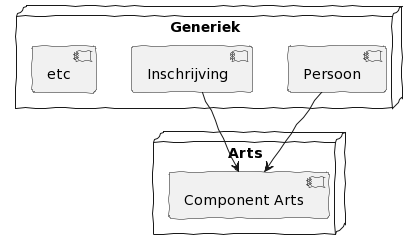
\includegraphics[width=0.4\textwidth]
        {arts.png}
     \caption{Arts with generiek}
     \label{fig:arts-deploy}
 \end{figure}
 \hfill
 \begin{figure}[h]
     \centering
     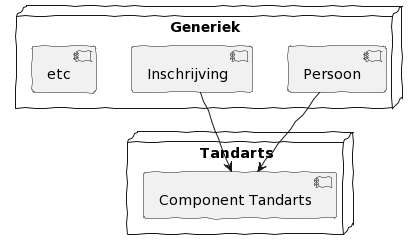
\includegraphics[width=0.4\textwidth]
        {tandarts.png}
    \caption{Tandarts with generiek}
    \label{fig:tandarts-deploy}
 \end{figure}
\\
Then the first professional group was removed from the database and the common data was also removed and the second group was fully initiated.
The method of building specific professional registers in this way is not (yet) supported by Ampersand, so it has to deployed all in once (\ref{fig:monoliet-deployment}).
\begin{figure}[H]
    \centering
        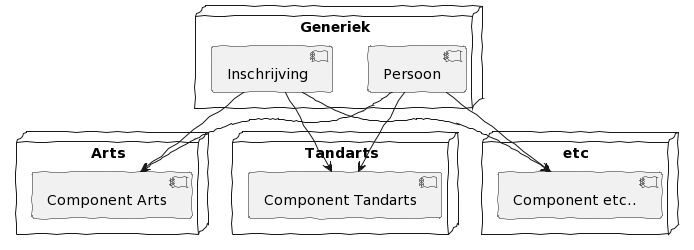
\includegraphics[width=1\textwidth]
            {monoliet.png}
        \caption{Deployment in once}
    \label{fig:monoliet-deployment}
\end{figure}
If this does not work for this law, it will also not work for links with other registers where data and the associated management software must be shared.
(Ref. to \nameref{s:3_2_common_objects})


\subsubsection{Authorization mechanism}\label{subsub:1_authorization_mechanism}
Every organization has an authorization mechanism for the software.
The \acrshort{cibg} uses a JWT mechanism.
In the research I encountered an authorization mechanism when creating the Rules and when building the Interface.
I have not found out whether it is possible to integrate this with the organization its own authorization mechanism.
(Ref. to \nameref{s:3_3_crud})


\subsubsection{Conventions}\label{subsub:1_conventions}
To use Ampersand correctly, knowledge of relation algebra is required.
You use this algebra as a Software engineer to build rules and relationships.
The knowledge of multiplicity is indispensable when making rules and relationships.
The naming convention on this is partly present within Ampersand.
Some elements, such as pattern, are capitalized and Concepts always start with a capital letter.
For example, there are a number of fixed agreements, but there are no agreements about the use of, for example, relation names.
(Ref. to \nameref{s:2_1_naming}, \nameref{s:2_2_multiplicity}, \nameref{s:2_3_rules})

\subsubsection{Other knowledge}\label{subsub:1_other_knowledge}
The Software engineer needs limited knowledge of Latex and HTML to influence the \acrshort{ca}.
In many cases this is not necessary because Ampersand handles this excellently.
However, there are opportunities to intervene and provide direction here.
(Ref. to \nameref{s:4_2_conceptual_analysis})

\subsubsection{Includes}\label{subsub:1_includes}
The Software engineer must know how to control Ampersand in terms of the use of includes.
These includes control the \acrshort{ca}, but are also used when building the application.
If the include is not specified where they are needed the build will fail and if it is specified where it is not needed the build will go well.
The \acrshort{se} has the option to send the \acrshort{ca} with includes.
The development of extra functions that have not yet been included within Ampersand is done using PHP.
The Software engineer therefore needs knowledge of PHP to develop these functions and of course Ampersand to be able to actually deploy these functions.
(Ref. to \nameref{s:3_1_includes}, \nameref{s:3_4_php})

\subsubsection{Team}\label{subsub:1_team}
The team that Ampersand maintains and wants to expand is very active.
The involvement is also apparent from the rapid resolution of issues that occurred.
(Ref. to \nameref{s:1_1_setup})